%%
% @author Rachel Baumann
%

%%%%%%%%%%%%%%%%%%%%%%%%%%%%%%% Preamble %%%%%%%%%%%%%%%%%%%%%%%%%%%%%%%%%%%%%%

\documentclass[11pt]{article}
\usepackage[english]{babel}
\usepackage[latin1]{inputenc}
\usepackage{amsmath}
\usepackage{graphicx}
\usepackage{mathtools}
\usepackage{latexsym}
\usepackage{amssymb}
\usepackage{amsfonts}
\usepackage{amstext}
\usepackage{multicol}  				% for having multiple columns
\usepackage{amsxtra} 
\usepackage{algorithm2e}    	% allows for using the algorithm environment
\usepackage{amsthm} 		 			% for proof environment
\usepackage{tikz}   		  		% for graphs and diagrams
\usetikzlibrary{arrows} 	 		% arrows for diagrams
\usepackage{pgfplots} 		 		% for graphs
\usepackage{multirow}					% for tables
\usepackage{xcolor, colortbl}	% for colors
\usepackage{pdfpages}					% to include pdf documents

%%%%%%%%%%%%%%%%%%%%%%%%%%%%%% New Command %%%%%%%%%%%%%%%%%%%%%%%%%%%%%%%%%%%%%

\newcommand{\ra}{\rightarrow}

%%%%%%%%%%%%%%%%%%%%%%%%%%%%%%%  Margins %%%%%%%%%%%%%%%%%%%%%%%%%%%%%%%%%%%%%%%%

\setlength{\topmargin}{-0.5in}        %%%  This sets all the spacing stuff to use the page more
\setlength{\oddsidemargin}{-0.5in}    %%%  efficiently than the normal "article" setup would.
\setlength{\evensidemargin}{-0.5in}   %%%  It's OK to play with these some.
\setlength{\textheight}{9.5in}     		%%%
\setlength{\textwidth}{7in}        		%%%
\setlength{\headsep}{0in}          		%%%
\setlength{\headheight}{0in}       		%%%

%%%%%%%%%%%%%%%%%%%%%%%%%%%%%%%%  document  %%%%%%%%%%%%%%%%%%%%%%%%%%%%%%%%%%%%%

\begin{document}

\begin{center}
{\Large \bf Sample Homework}\\
 \ \\
	{\large YOUR NAME HERE}\\{\today}
\end{center}

\vspace{0.5cm} 	% vertical space


%%%%%%%%%%%%%%%%%%%%%%%%%%%%%%%% Math Reivew %%%%%%%%%%%%%%%%%%%%%%%%%%%%%%%%%

{\large\textbf{Math Review}}

\begin{enumerate}
\item[1.] First to use the math environment to insert and equation or formula use the single or double dollar signs about the expression like so: $3x + 5x^2 = 8$ or 

$$3x+5x^2 = 8.$$

To create an equation on multiple lines use the `align' environment:

\begin{align*}
4(x+3) - 3(-x-2) & = 4x + 12 -3(-x) -3(-2) \quad \text{[By Distributive Law]}\\
&= 4x+12 + 3x + 6 \quad \text{[By Associative Law]}\\
&= 7x + 18 \quad \text{[By commutative Law]}
\end{align*}


\item[2.] Here are some basic math commands in the .tex file and their outputs in the .pdf file:

For fractions: $$\frac{1}{2} \cdot \frac{1+x + x^2}{x^3 + x + 4}$$

For summation and product notation: 

$$\sum_{i = 0}^{n+1} (i^2 + 2) \quad \text{and} \quad \prod_{i=0}^{n-1} i + 3 \quad \text{and} \quad \left(\sum_{i=-n}^n i^2 \right)$$

For square roots: $\sqrt{2}, ~ \sqrt{10 - x^2}$, $n^{th}$ roots: $\sqrt[n]{1+x+x^2}$\\

For logarithms and exponents: $\log_3 (x^4)$, $4^{\log_4 x}$\\

Inequalities: $x\geq 0$ and $x \leq 0$\\

To create a list of numbers: $\qquad \dots, ~ -1, ~ 0, ~ 1, ~2, ~ 3, ~ \dots$

Sets of numbers: $$\mathbb{R},\quad \mathbb{Z}^+, \quad \mathbb{Q}_{\geq 0}, \quad \{0,~1,~2, ~3\}, \quad \{x \in \mathbb{Z} \mid x \geq 0 \} = \mathbb{Z}_{\geq 0}$$

Basic set operators: $A \cap B, \quad A \cup B, \quad A- B,\quad  \overline{A} = U - A, \quad A\subseteq B, \quad A \supset B$ \\

Power set: $\mathcal{P}(\emptyset) = \{\emptyset,~ \{\emptyset\}\}$\\

Boxing your solutions:

\begin{equation*}
 \boxed{x^2+y^2 = z^2}
\end{equation*}
\end{enumerate}

%%%%%%%%%%%%%%%%%%%%%%%%%%%%%%%%%%%% Section 1.1 %%%%%%%%%%%%%%%%%%%%%%%%%%%%%%%%%


{\large\textbf{Section 1.1 - Logic}}\newline

Some logic symbols:

\begin{multicols}{2}
\begin{itemize}
\item AND: $\land$

\item OR (inclusive): $\lor$

\item XOR (exclusive): $\oplus$

\item Negation: $\lnot$

\item Equivalence: $\equiv$

\item Implication: $\leftarrow$, $\rightarrow$, $\Rightarrow$
\end{itemize}

\begin{itemize}
\item Biimplication: $\leftrightarrow$ or $\Leftrightarrow$

\item True and False: \textbf{T} and \textbf{F}

\item Universal Quantification: $\forall$

\item Existential Quantification: $\exists$

\item Therefore: $\therefore$


\end{itemize}
\end{multicols}
 
\vspace{0.5cm}


%%%%%%%%%%%%%%%%%%%%%%%%%%%%%% Section 1.7 %%%%%%%%%%%%%%%%%%%%%%%%%%%%%%%%

{\large\textbf{Section 1.7 - Proofs}}

\begin{enumerate}
\item Prove that if $x \in \mathbb{Z}$ is even, then $x^2 + 1$ is odd.


\begin{proof}
(Direct): \\

Let $x\in \mathbb{Z}$ and suppose that $x$ is even. Then by definition $x = 2k$ for some $k \in \mathbb{Z}$. Next consider $x^2 + 1$.
\begin{align*}
x^2+ 1 & = (2k)^2 + 1\\
&= 4k^2 + 1\\
&= 2(2k^2) + 1
\end{align*}
Since $n=2k^2 \in \mathbb{Z}$ we have that $x^2+1 = 2n + 1$ for $n \in \mathbb{Z}$ and hence by definition $x^2 + 1$ is add.
\end{proof}



\item Prove or disprove: the subtraction of two irrational numbers is irrational.\\

\textit{Disproof}. (Counterexample):\\

Consider $\sqrt{2}$  which is irrational. However 

$$\sqrt{2} - \sqrt{2} = 0$$

and as $0 \in \mathbb{Q}$ this contradicts the statement above, hence it is false.\\


\end{enumerate}


%%%%%%%%%%%%%%%%%%%%%%%%%%%%%%%% Section 2.3 %%%%%%%%%%%%%%%%%%%%%%%%%%%

\newpage % start on a new page

{\large\textbf{Section 2.3 - Functions}}\\

Floor function: $\lfloor x \rfloor$\\

Ceiling function: $\lceil x \rceil$\\

Functions composition: $f \circ  g: \mathbb{Z} \rightarrow \mathbb{Z}$\\

Piecewise Functions:

$$ f(n) = \left\{ 
  \begin{array}{l l}
    \frac{n}{2} & \quad \text{if $n$ is even}\\
    -\frac{n+1}{2} & \quad \text{if $n$ is odd}
  \end{array} \right.$$


Graphing:

\begin{center}
\begin{tikzpicture}[>=stealth]
    \begin{axis}[
        xmin=-4,xmax=4,
        ymin=-2,ymax=2,
        axis x line=middle,
        axis y line=middle,
        axis line style=<->,
        xlabel={$x$},
        ylabel={$y$},]
        \addplot[no marks,blue, <->] expression[domain=-pi:pi,samples=100]{x^2+x-1} 
                    node[pos=0.65,anchor=south west]{$y=x^2-x-1$}; 
    \end{axis}
\end{tikzpicture}\\
\textbf{Figure :} Graph of $f(x) = x^2+x-1$
\end{center}

\vspace{0.5cm}


\begin{center}\small{
    \begin{tikzpicture}
    \draw[gray!50, thin, step=1] (-3,-2) grid (7,6);
    \draw[very thick,->] (-3,0) -- (7,0) node[right] {$x_1$};
    \draw[very thick,->] (0,-2) -- (0,6) node[above] {$x_2$};
    \foreach \x in {-3,...,7} \draw (\x,0.05) -- (\x,-0.05) node[below] {\tiny\x};
    \foreach \y in {-2,...,6} \draw (-0.05,\y) -- (0.05,\y) node[right] {\tiny\y};
    \fill[green!50!green,opacity=0.3] (0,6) -- (7,6) -- (7,4) -- (9/16,13/16) -- (0,2)--  cycle;
    \draw (-3,-1) -- node[above right, sloped] {\small$x_1 \geq \frac{1}{2}x_2 + \frac{1}{2}$} (7, 4);
    \draw (-2,6)  -- node[above right, sloped] {\small$x_1 \geq 2 - 2x_2$} (2,-2);
    \end{tikzpicture}}
\end{center}
	


\newpage

%%%%%%%%%%%%%%%%%%%%%%%%%%%%%% Section 2.6 %%%%%%%%%%%%%%%%%%%%%%%%%%%%%%%%%%


{\large\textbf{Section  2.6 - Matrices}}\\

For each part of this problem below, consider the matrices:

$$A= \begin{bmatrix}
1 & 2\\
0 & 1
\end{bmatrix}
\quad
B = \begin{bmatrix}
3 & 4 & -1\\
-5 & 7 & 0
\end{bmatrix}
\quad
C = \begin{bmatrix}
-1 & 0\\
0 & 1
\end{bmatrix}
$$

\begin{enumerate}
\item[(a)] Compute $A+C$.

$$A+C = \begin{bmatrix}
1 & 2\\
0 & 1
\end{bmatrix}
+ 
\begin{bmatrix}
-1 & 0\\
0 & 1
\end{bmatrix}
=
\begin{bmatrix}
0 & 2\\
0 & 2
\end{bmatrix}
$$



\item[(b)] Compute $A\cdot B$.

$$A\cdot B = \begin{bmatrix}
1 & 2\\
0 & 1
\end{bmatrix}
\cdot
\begin{bmatrix}
3 & 4 & -1\\
-5 & 7 & 0
\end{bmatrix}
=
\begin{bmatrix}
-7 & 18 & -1\\
-5 & 7 & 0
\end{bmatrix}
$$

\item[(c)] Compute $C^2$.

$$C^2 = \begin{bmatrix}
-1 & 0\\
0 & 1
\end{bmatrix}
\cdot \begin{bmatrix}
-1 & 0\\
0 & 1
\end{bmatrix}
=
\begin{bmatrix}
1 & 0\\
0 & 1
\end{bmatrix}
$$

\item[(d)] Compute $I_3 \odot I_3 \odot I_3$.

$$I_3 \odot I_3 \odot I_3 = I_3 \odot I_3 = I_3$$

\end{enumerate}


A general $m \times n$ matrix:

$$
A_{m,n} =
 \begin{pmatrix}
  a_{1,1} & a_{1,2} & \cdots & a_{1,n} \\
  a_{2,1} & a_{2,2} & \cdots & a_{2,n} \\
  \vdots  & \vdots  & \ddots & \vdots  \\
  a_{m,1} & a_{m,2} & \cdots & a_{m,n}
 \end{pmatrix}
$$


\newpage


%%%%%%%%%%%%%%%%%%%%%%%%%%%%%%%%%%%% Section 3.1 %%%%%%%%%%%%%%%%%%%%%%%%%%%%%%%%


{\large\textbf{Section 3.1 - Algorithms}}

\begin{itemize}

\item To write code in LaTeX that looks like actual code use verbatim:

\begin{enumerate}
\item[] \begin{verbatim}
for i in range(1, 5):
  print i
else:
  print "The for loop is over"
\end{verbatim}
\end{enumerate}

\item To write an algorithm in pseudo code use the algorithm 2e package, which is already in the preamble,\\

\begin{algorithm}[H]
 \SetAlgoLined
 \KwData{this text}
 \KwResult{how to write algorithm with \LaTeX2e }
 initialization\;
 \While{not at end of this document}{
  read current\;
  \eIf{understand}{
   go to next section\;
   current section becomes this one\;
   }{
   go back to the beginning of current section\;
  }
 }
 \caption{How to write algorithms}
\end{algorithm}

\vspace{0.3cm}

\item Here is another example:\\

\fbox{\parbox{10cm}{%
\begin{tabbing}
    {\tt 1}  \ \ \textbf{PrintAll}( node $v$ ):\\
    {\tt 2}  \ \ \ \ \ \ for each (item in $v$ as $x$ in order) \{ \ \ \ \\
    {\tt 3}  \ \ \ \ \ \ \ \ \ \ if $x ==$ is a key \\
    {\tt 4}  \ \ \ \ \ \ \ \ \ \ \ \ \ \ print $x$ \\
    {\tt 5}  \ \ \ \ \ \ \ \ \ \ else PrintAll($x$)\\
    {\tt 6}  \ \ \ \ \ \ \};
\end{tabbing}
}}

\end{itemize}

\vspace{0.5cm}


%%%%%%%%%%%%%%%%%%%%%%%%%%%%%%%%%%% Section 6.4 %%%%%%%%%%%%%%%%%%%%%%%%%%%%%%%%%%


{\large\textbf{Section 6.4 - Counting}}\\

Permutations: $$P(n,r) = \frac{n!}{(n-r)!} = {n\choose r} \cdot r!$$

Combinations: $$C(n,r) = \frac{n!}{r!(n-r)!} = \binom{n}{r}$$



\newpage

%%%%%%%%%%%%%%%%%%%%%%%%%%%%%%%%% Section 9.1 %%%%%%%%%%%%%%%%%%%%%%%%%%%%%%


{\large\textbf{Section 9.1 - Relations}}\\

Comparable: $\succeq	$, $\preceq$\\

\noindent
Here are some graph representations of relations, the first one is the kind we'll use in this course whereas the second you may see in Discrete Structures or Algorithms. I just included it to give you more options.



\begin{center}
\begin{tikzpicture}[->,>=stealth',shorten >=1pt,auto,node distance=3cm,
  thick,main node/.style={circle,fill=blue!20,draw,font=\sffamily\Large\bfseries}]

  \node[main node] (1) {1};
  \node[main node] (2) [below left of=1] {2};
  \node[main node] (3) [below right of=2] {3};
  \node[main node] (4) [below right of=1] {4};

  \path[every node/.style={font=\sffamily\small}]
    (1) edge node [left] {} (4)
        edge [bend right] node[left] {} (2)
        edge [loop above] node {} (1)
    (2) edge node [right] {} (1)
        edge node {} (4)
        edge [loop left] node {} (2)
        edge [bend right] node[left] {} (3)
    (3) edge node [right] {} (2)
        edge [bend right] node[right] {} (4)
    (4) edge node [left] {} (3)
        edge [loop right] node {} (4)
        edge [bend right] node[right] {} (1);
\end{tikzpicture}\\
 \textbf{Figure 1: } Relation of the set $\{1,~2,~3,~4\}$
\end{center}

\vspace{0.5cm}

\begin{center}
\begin{tikzpicture}[->,>=stealth',shorten >=1pt,auto,node distance=3cm,
                    thick,main node/.style={circle,draw,font=\sffamily\Large\bfseries}]

  \node[main node] (1) {s};
  \node[main node] (2) [above right of=1] {$v_1$};
  \node[main node] (3) [below right of=1] {$v_2$};
  \node[main node] (4) [right of=2] {$v_3$};
  \node[main node] (5) [right of=3] {$v_4$};
  \node[main node] (6) [below right of=4] {t};

  \path[every node/.style={font=\sffamily\small}]
    (1) edge [bend left] node[left] {4} (2)
        edge [bend right] node[left] {2} (3)
    (2) edge [bend left] node[above left] {12} (1)
    (3) edge [bend right] node[below] {3} (5)
        edge node {4} (2)
        edge [bend right] node[below left] {11} (1)
    (4) edge node[left] {9} (3)
        edge [bend left] node {1} (6)
        edge node[above] {12} (2)
        edge node {7} (5)
    (5) %edge node {7} (4)
    	edge [bend right] node {11} (3)
        %edge [bend right] node[below right] {4} (6)
    (6) edge [bend left] node[above right] {19} (4)
    	edge [bend left] node[below right] {4} (5);
					
\end{tikzpicture}\\
 \textbf{Figure 2: } Network Flow

\end{center}


\newpage


%%%%%%%%%%%%%%%%%%%%%%%%%%%%% Greek %%%%%%%%%%%%%%%%%%%%%%%%%%%%%%


{\large\textbf{Greek Letters}}

\begin{multicols}{2}
\begin{itemize}
\item alpha: $A$, $\alpha$

\item beta: $B$, $\beta$

\item gamma: $\Gamma$, $\gamma$

\item delta: $\Delta$, $\delta$

\item epsilon: $E$, $\epsilon$

\item theta: $\Theta$, $\theta$
\end{itemize}

\begin{itemize}
\item Lambda: $\Lambda$, $\lambda$

\item mu: $M$, $\mu$

\item sigma: $\Sigma$, $\sigma$

\item phi: $\Phi$, $\phi$

\item psi: $\Psi$, $\psi$

\item omega: $\Omega$, $\omega$
\end{itemize}
\end{multicols}

\vspace{0.5cm}

{\large\bf Calculus}


\begin{enumerate}
\item Limits:

$$\lim_{x \ra 0^+} \frac{\sin x}{x} = 1 \quad\text{ and }\quad \lim_{x \ra 0^-}\frac{\sin x}{x} = 1 \quad\text{ thus } \quad\lim_{x \ra 0} \frac{\sin x}{x} =1$$


\item Derivative Notation:

$$y'= f'(x) = \frac{df}{dx} = \frac{dy}{dx}=\frac{d}{dx} f(x) $$

$$y'' = f''(x) = \frac{d^2 f}{dx^2} = \frac{d^2y}{dx^2} = \frac{d^2}{dx^2} f(x)$$


\item Integrals:

$$\int \cos x ~ dx = \sin x + C$$
$$\int_0^2 x ~dx = 2 $$

\item Symbols:

\begin{itemize}
\item Partial: $\partial$
\item Delta: $\Delta$
\end{itemize}



\end{enumerate}


\end{document}
